% Created 2021-10-28 Thu 03:45
% Intended LaTeX compiler: pdflatex
\documentclass[a4paper]{article}
\usepackage[utf8]{inputenc}
\usepackage[T1]{fontenc}
\usepackage{graphicx}
\usepackage{grffile}
\usepackage{longtable}
\usepackage{wrapfig}
\usepackage{rotating}
\usepackage[normalem]{ulem}
\usepackage{amsmath}
\usepackage{textcomp}
\usepackage{amssymb}
\usepackage{capt-of}
\usepackage{hyperref}
\documentclass{article}
\usepackage{here}
\usepackage{xcolor}
\usepackage[margin=3.0cm]{geometry}
\usepackage{amsmath}
\usepackage{parskip}
\renewcommand\arraystretch{1.4}
\usepackage[margin=1in]{geometry}
\usepackage{minted}
\usepackage{multicol}
\definecolor{bg}{rgb}{0.95,0.95,0.95}
\newminted{java}{fontsize=\footnotesize,frame=single,framesep=2mm}
\newminted{text}{breaklines,fontsize=\footnotesize,frame=single,framesep=2mm}
\author{Fatih Kaan Salgır - 171044009}
\date{}
\title{CSE443 - Object-Orianted Analysis \& Desing - HW 1}
\hypersetup{
 pdfauthor={Fatih Kaan Salgır - 171044009},
 pdftitle={CSE443 - Object-Orianted Analysis \& Desing - HW 1},
 pdfkeywords={},
 pdfsubject={},
 pdfcreator={Emacs 27.2 (Org mode 9.5)}, 
 pdflang={English}}
\begin{document}

\maketitle

\section*{Design Explanation}
\label{sec:org7fe60f4}

\subsection*{Java Swing Platform Game}
\label{sec:orge33f708}

\texttt{Main} class creates a \texttt{JFrame} and sets its content pane to new \texttt{GamePanel}.
\texttt{Gamepanel} extends \texttt{Jpanel} and implements;
\begin{itemize}
\item \texttt{Runnable}: for creting game loop.
\item \texttt{KeyListener}: for listening keys press and relases. \texttt{HashMap<Integer, Boolean> keyPressed} with \texttt{registerKeyEvent} is used to keep track of keys.
\end{itemize}
Whenever the keys are pressed the value of the corresponding key in the hash map set to \texttt{true}.
\begin{itemize}
\item \texttt{MouseListener}: for listening clicks on the pane to check whether the user clicked the pause button.
\end{itemize}


Game loop targets the 60 FPS.
Checks the collisions, earned points, power-up acqusitions, key presses, and update the state accordingly.
Updates the positions of the each view and HUD and draws into \texttt{BufferedImage}.
If still there is time before drawing the next frame, the thread sleeps for a number of calculated miliseconds to target 60 FPS.

Lower part of the window is left for debug messages.
\texttt{JList} with \texttt{DefaultListModel<String>} is used on top of \texttt{ScorllPane}, so whenever a log is added to the \texttt{DefaultListModel}, it is displayed in the \texttt{JList}.

\texttt{common/Util.java} stores the constants used different classes like the width \& height of the window, position \& sizes of objects, file paths etc.


\newpage
\subsection*{Decorator Pattern}
\label{sec:orgc7205b9}

Decorater pattern demonstration in game loop;

In \texttt{GamePanel.java}:

\begin{javacode}
private Multiplier multiplier;
// ...
this.multiplier = new BaseMultiplier();
// ...

// on successfull jump
score += multiplier.unitPoints();

// when new power-up acquired
switch (p.type) {
    case A:
        multiplier = new PowerUpA(multiplier);
        // ...
    break;
    case B:
        multiplier = new PowerUpB(multiplier);
        // ...
    break;
    case C:
        multiplier = new PowerUpC(multiplier);
        // ...
    break;
    // ...

}
\end{javacode}


\begin{figure}[htbp]
\centering
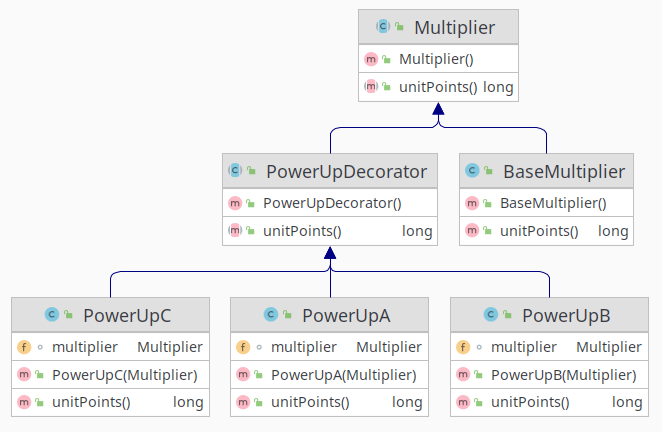
\includegraphics[width=300px]{org-img/Design_Explanation/2021-10-28_02-08-52_screenshot.png}
\caption{Desing of the Power-up Modal Classes}
\end{figure}


\newpage
\subsection*{Strategy Pattern}
\label{sec:orgb94f953}

In game loop there are three methods need to be used to manage any jump behaviour.
These are \texttt{jump()}, \texttt{updatePosition()} and \texttt{isJumping()} which is defined as abstract methods in \texttt{JumpBehaviour}.
Therefore any jump, must implement these functions.
\texttt{Actor} is an abstract class which only consists of methdos that calls \emph{behaviour} methods and getter/setter for the jump behaviour.
Whenever the \texttt{Actor} methods are called, methods of the \texttt{JumpBehaviour} will be called.


\texttt{JumpPhysic} is only a helper class to calculate character's next position according to elapsed time simulating gravitational acceleration.
Whenever the jump mode changes, also the initial velocity changes.
Depending on the inital velocity, time in the air also changes.
Since the power-up D is acquired when jumping, the behaviour doesn't change immediately but prempted till the jump is over.



Dynamically changing the jump type:

In \texttt{GameCharacter.java};

\begin{javacode}
// ...
public void toggleJumpMode() {
  if (getJumpBehaviour() instanceof JumpLow) {
    nextJumpBehavior = new JumpHigh(this.characterView);
    characterView.setImage(Util.CHARACTER_WITH_WINGS_FILENAME);
  } else {
    nextJumpBehavior = new JumpLow(this.characterView);
    characterView.setImage(Util.CHARACTER_FILENAME);
  }
}

@Override
public void updatePosition(long start) {
  jumpBehaviour.updatePosition(start);
  if (nextJumpBehavior != null && !isJumping()) {
    setJumpBehaviour(nextJumpBehavior);
  }
}

// ...
\end{javacode}

\begin{figure}[htbp]
\centering
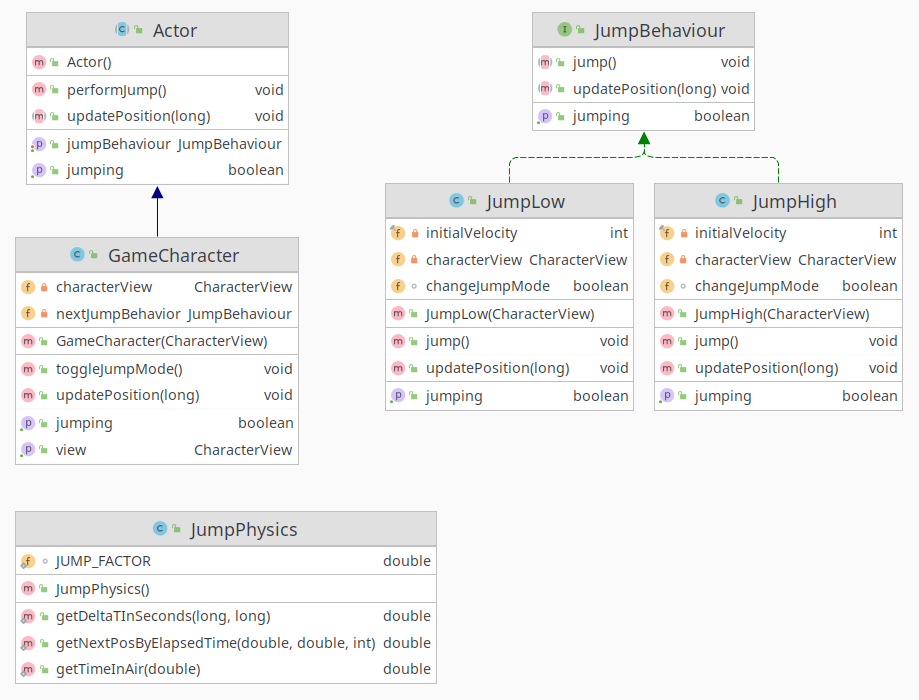
\includegraphics[width=300px]{org-img/Design_Explanation/2021-10-28_02-05-29_screenshot.png}
\caption{Desing of the JumpBaheviour \& Actor Classes}
\end{figure}




\newpage
\subsection*{Views}
\label{sec:org3785fd3}

Everything that is drawed in the pane is collected into \texttt{View} package.

\begin{center}
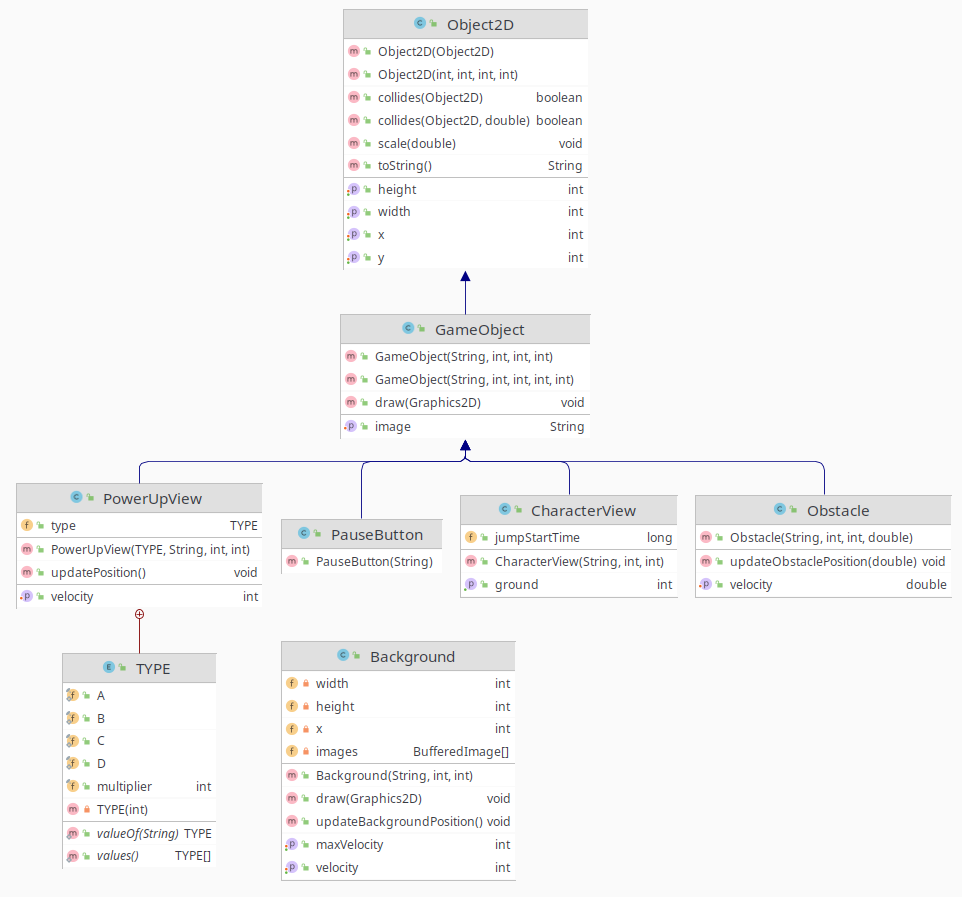
\includegraphics[width=.9\linewidth]{org-img/Design_Explanation/2021-10-28_02-11-11_screenshot.png}
\end{center}

\subsection*{Play / Pause}
\label{sec:orge6a0e1a}

When the game is paused the only state should be saved is the position of the main character.
The only parameter which sets the character position is the current time and start time of the jump.
So start time of the jump is saved when the game paused and restored as \textbf{current time \(-\) time in the air when paused}.

\subsection*{Notes}
\label{sec:org61ee81d}

\begin{itemize}
\item In order to get better game experince; collision detection thershold with obstacles is decreased, and thershold with power-ups is increased.
\end{itemize}


\newpage
\subsection*{General Class Diagram}
\label{sec:orge1ffedc}

\begin{center}
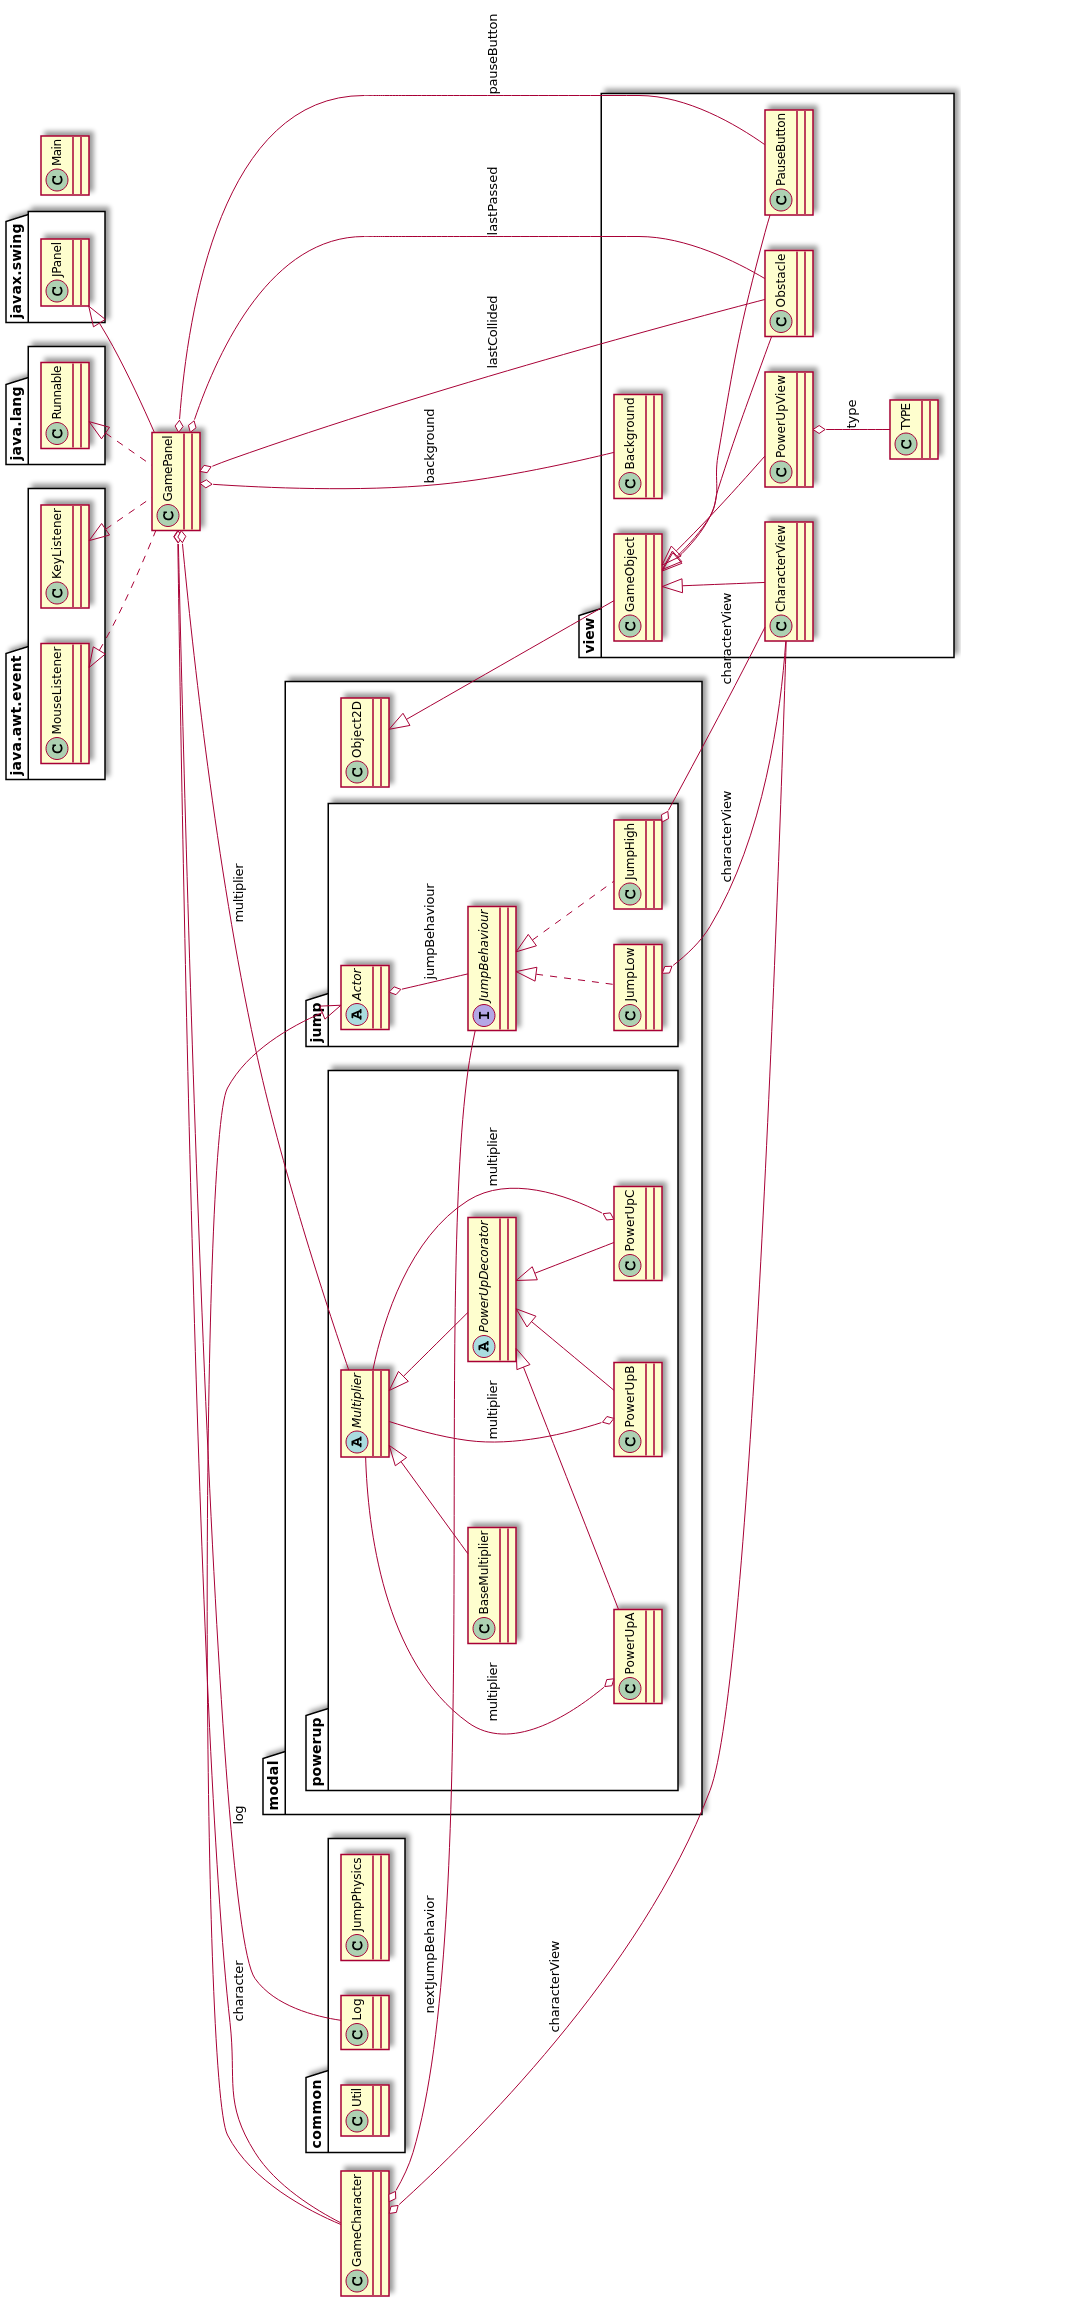
\includegraphics[width=300px]{org-img/Design_Explanation/2021-10-28_03-43-15_screenshot.png}
\end{center}
\end{document}
